\chapter{WEB应用开发及持续集成}
\label{cha:web}
本论文的研究目的是对开发的WEB应用在应用、数据库和服务器层级进行优化,通过对比不同优化策略对于系统性能提升的影响研究一套可行的系统优化方案。为了实现优化的目的,首先需要创建一个WEB应用或者对现有的应用进行优化,本人在研究生期间,参与了海信集团智能商用公司的小微商户平台系统的开发,主要工作是后台开发和服务器运维工作,因此本论文将基于该项目进行系统优化策略的研究。

在优化之前,首先需要描述作为优化原型的小微商户WEB平台的开发框架以及应用部署流程。

% 本章首先介绍WEB应用开发的主要程序语言,然后对Spring MVC框架进行了详细的介绍。同时,对各种技术的应用反问做了初步的探讨,为后文系统性能优化工作做好理论工具上的准备。
% \section{应用开发语言}
% 目前WEB应用开发主要分为前端开发和后端开发,其中前端开发以HTML和JavaScript结合为主,后端开发语言则比较多,主流的有C语言、PHP语言、JAVA语言以及Python语言等语言,不同语言之间的作用和特点都不同,但在提高系统稳定性和系统兼容性方面JAVA语言更有优势~\cite{suzumura2008performance}。
% \subsection{JAVA语言}
% \subsubsection{JAVA语言产生及发展}
% JAVA语言是在20世纪90年代产生的,任职于太阳微系统的詹姆斯·高斯林等人于1990年代初开发Java语言的雏形,最初被命名为Oak,目标设置在家用电器等小型系统的程序语言,应用在电视机、电话、闹钟、烤面包机等家用电器的控制和通信~\cite{byous1998java}。由于这些智能化家电的市场需求没有预期的高,Sun公司放弃了该项计划。随着1990年代互联网的发展,Sun公司看见Oak在互联网上应用的前景,于是改造了Oak,于1995年5月以Java的名称正式发布。Java伴随着互联网的迅猛发展而发展,逐渐成为重要的网络编程语言~\cite{java维基百科}。

% 在所有的编程语言中,应用最广泛的莫过于JAVA语言,该语言在面向对象的程序开发中一直有着突出的表现。因此在最近10几年间,JAVA语言一直保持在编程语言排行的前两名,参见图~\ref{fig:tiobe}。
% \begin{figure}[H] % use float package if you want it here
%   \centering
%   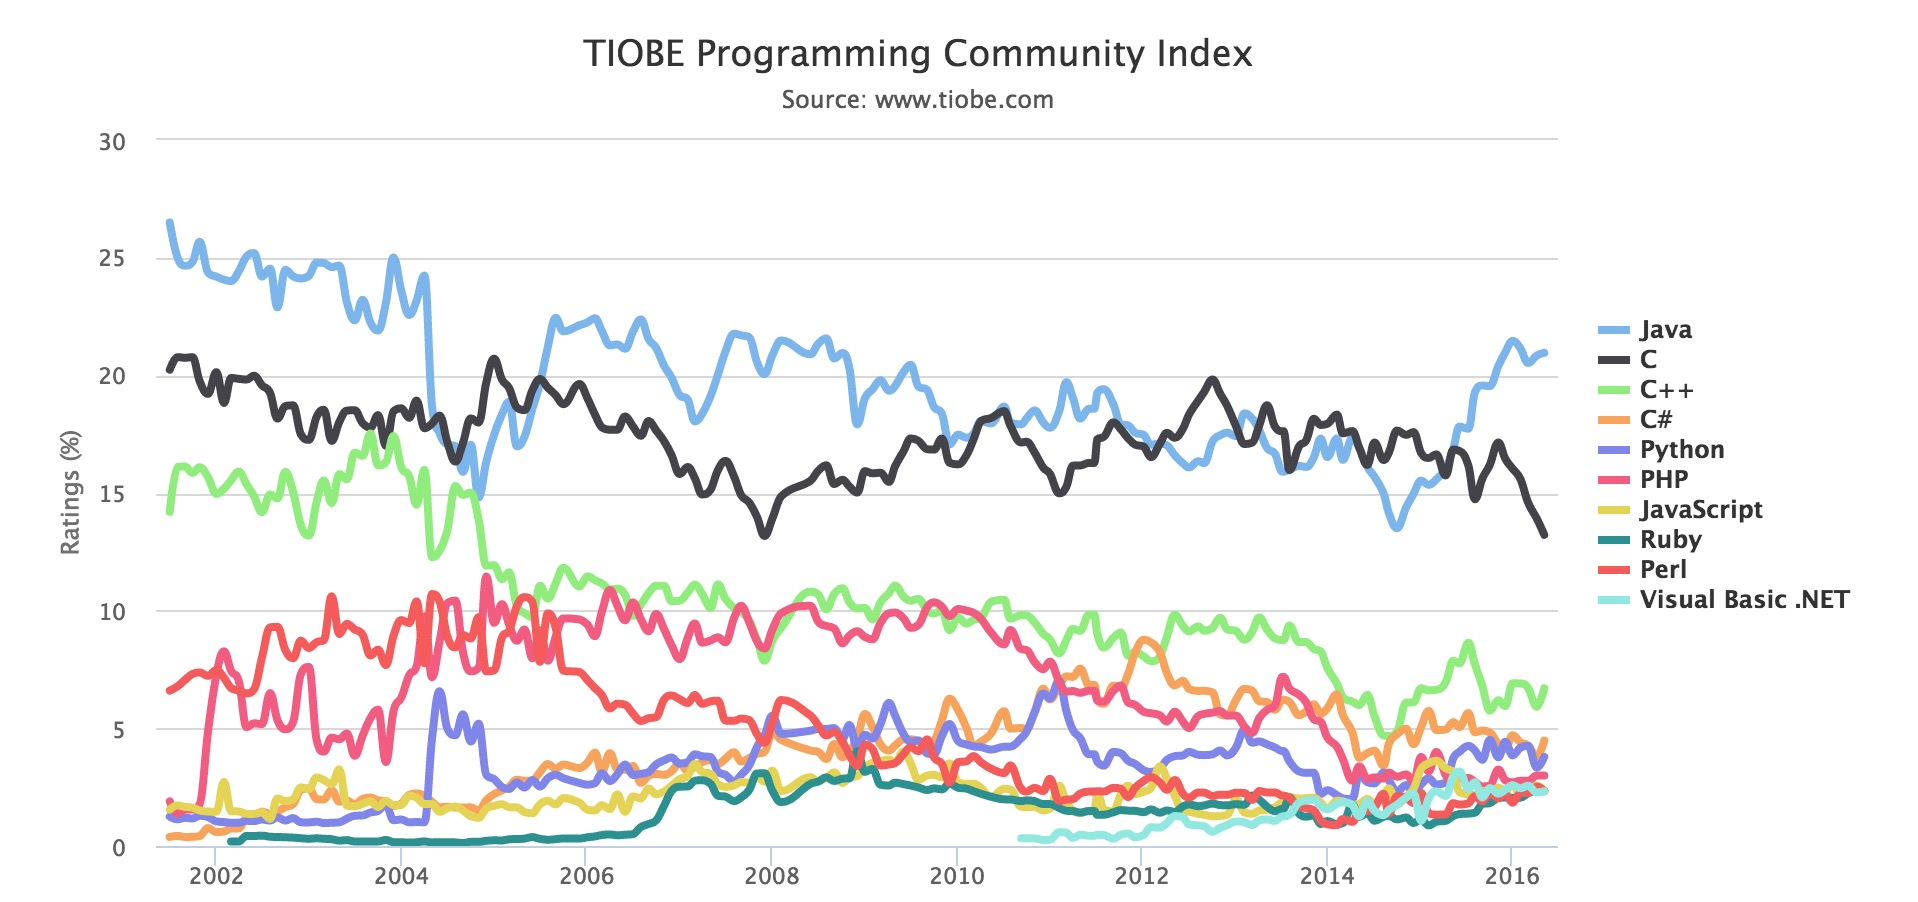
\includegraphics[width=6in]{chap02/1-TIOBE}
%   \caption{编程语言近年排行}
%   \label{fig:tiobe}
% \end{figure}
% \subsubsection{JAVA语言特点}
% 因特网的普及推动了JAVA语言的发展,同时JAVA语言在网页制作上的应用也丰富了因特网的内容。两者可谓是相辅相成、相互促进。JAVA语言的特点如表\ref{tab:java-1}。
% \begin{table}[htb]
%   \centering
%   \begin{minipage}[t]{0.8\linewidth} % 如果想在表格中使用脚注,minipage是个不错的办法
%   \caption[模板文件]{模板文件。如果表格的标题很长,那么在表格索引中就会很不美
%     观,所以要像 chapter 那样在前面用中括号写一个简短的标题。这个标题会出现在索
%     引中。}
%   \label{tab:java-1}
%     \begin{tabularx}{\linewidth}{lX}
%       \toprule[1.5pt]
%       {\heiti 特点} & {\heiti 描述} \\\midrule[1pt]
%       可移植性 & 能移植于不同的使用平台,扩大了系统的使用范围 \\
%       面向对象 & 集成了C++的优点,并且在面向对象方面有新的扩展 \\
%       多线程 & 可以让多个不同处理器同时进行工作,是数据库系统开发的最佳选择 \\
%       分布式 & 在处理TCP等协议的同时也支持网络编程\\
%       \bottomrule[1.5pt]
%     \end{tabularx}
%   \end{minipage}
% \end{table}


\section{Spring MVC开发框架}

Spring MVC 开发框架是一种针对Java语言开发的WEB系统架构,该框架的设计理念是对开发的系统整体进行分解,通过不同的方式对分解后的工作进行处理,以更加专业的技术解决具体的问题,最终在不同的模块中通过调用实现系统的整体呈现,通过这种方法可使系统的耦合度同其他的框架如Struts相比大大的降低。\cite{林薇2015基于}。
% \subsection{Spring MVC 架构的特点}
% Spring MVC 架构不同于传统的体系架构,在其发展的过程中吸收其他系统的特点,如支持Userful风格,灵活的本地化等。这些特征保证了Spring MVC框架在发展过程中,更加受到开发者的青睐。同时,吸收了前人的经验以后,Spring MVC框架也具备专属的特点,比如用Spring MVC框架设计的WEB系统其耦合度较低,系统总体表现出简洁明了的风格,这样用户就能更快捷的掌握数据库系统的操作~\cite{林薇2015基于}。

% Spring MVC框架是在Spring框架的基础上发展起来的,因此Spring MVC框架集成了Spring 框架的所有功能,而且两者在相互继承方面表现出很好的融合性。这一特点给系统开发带来了很多方便。除此之外,Spring MVC模型在图形兼容性和数据验证的灵活性上都有先天的优势。正式因为这些特点,使Spring MVC模型在实际应用中发挥出巨大的优势,同时也在程序员中受到青睐。本文的WEB应用就是建立在该框架之上的\cite{林薇2015基于}。
\subsection{Spring MVC 框架处理流程}

本框架是一个基于用户请求的系统架构。框架的处理过程参见图~\ref{fig:mvc},反映了一个简单的从用户请求开始到获得响应的过程。

\begin{figure}[H] % use float package if you want it here
  \centering
  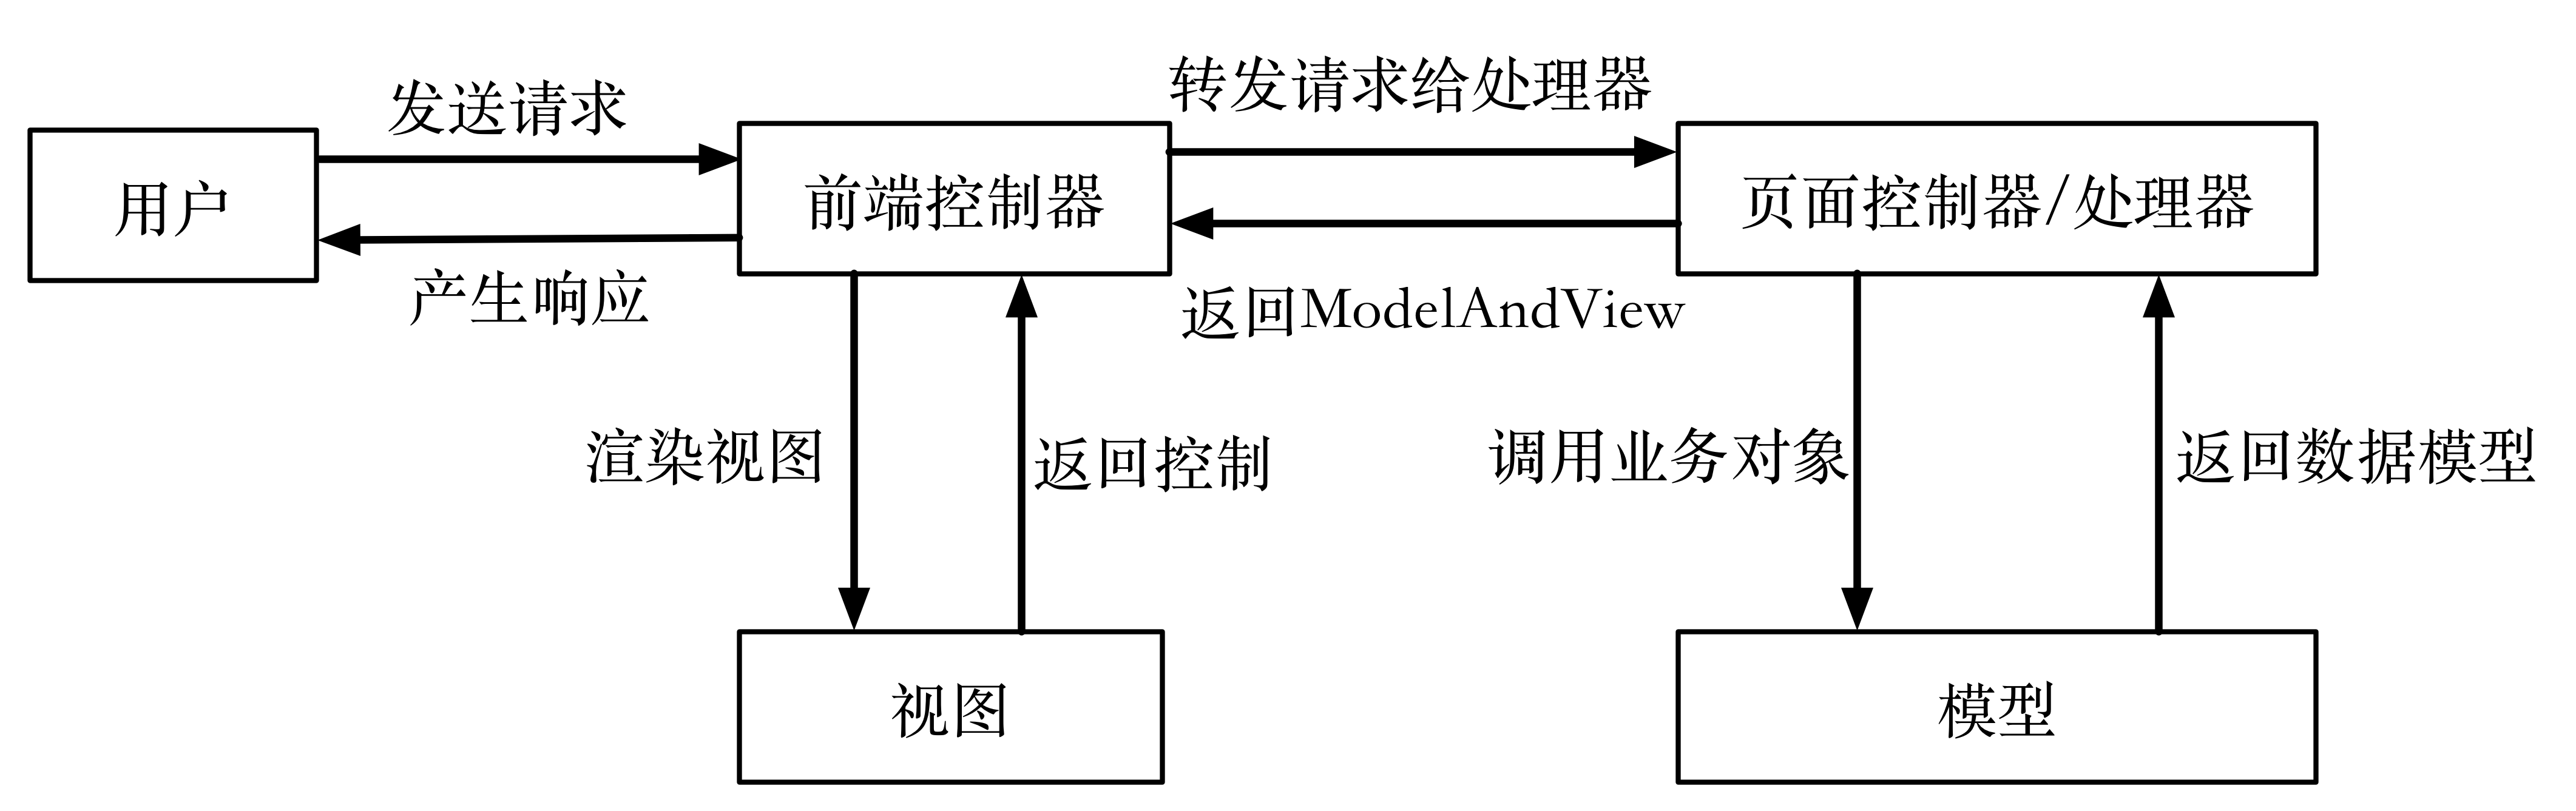
\includegraphics[width=6in]{chap02/mvc}
  \caption{Spring MVC请求响应过程}
  \label{fig:mvc}
\end{figure}

通过图可以看出,首先需要用户发送请求到框架的前端控制器,前端控制器接收到用户请求后会对用户的请求内容进行分析,获取到请求的控制器地址和请求参数,根据请求地址将用户请求转发到对应的后端控制器即处理器。处理器在接收到请求的参数之后开始调用后台的业务对象对请求进行分析和处理,在处理过程中会通过模型对存在数据库中的数据进行增、删、改、查的操作,处理完毕后将最新的数据返回给处理器;在请求的处理工作完成返回给前端控制器,之后对需要显示的结果进行视图渲染生成显示页面,展示给用户,对用户的请求产生了响应\cite{李守振2006web}。

\subsection{Spring MVC体系的三层架构}
Spring MVC开发框架的架构主要体现在MVC(Model View Controller),它是模型(M)、视图(V)和控制(C)三个英文单词的首字母缩写,本系统的架构分为模型层(数据访问层)、视图层和控制层三层。

\begin{enumerate}

\item 视图层。主要负责前端页面的用户请求,将用户请求按照URL Mapping方式映射到相对应的控制器,通过分析用户请求,Spring可以自动的去寻找响应该请求的控制类,当控制类处理完请求后会将请求的结果以用户指定方式显示在前端页面上。

\item 控制层。 控制层是架构中承上启下的一层,这一层的作用是接受视图层传来的用户请求,然后针对请求设计实现用户请求的方法,需要用到数据的则会通过模型层获取数据结果,通过算法处理获得用户请求的结果,并且将结果返回视图层。

\item 模型层,也可以成为数据访问层。这一层的作用主要是实现数据的访问方法和数据的返回方法,通过配置数据模型访问数据库并且获得需要的数据,将数据返回给控制层。

\end{enumerate}

以上的Spring MVC三层架构体系在很大程度上根据开发需求实现了业务的剥离,解决了开发过程中的开发资源和业务资源混乱的问题,而且降低了系统的耦合度。

\section{应用开发工具}

在开发基于 Spring MVC 的 WEB 应用过程中,需要用到的基础编程语言是 JAVA,系统的架构采用的是 MVC 三层架构。但是在架构之外,程序本身的开发对于研究人员也非常重要,因此通过选择和使用一些比较好用的软件和工具,对于缩短开发周期、提升开发效率来说非常重要。

\subsection{IntelliJ IDEA}

IntelliJ IDEA 是一款 Java 集中开发环境工具软件,由捷克软件公司 JetBrains 发布和维护~\cite{jemerov2008implementing}。

随着用户数量的增加和软件自身的优良特性,目前已经成为Java语言开发过程中效率最好的集成开发环境之一。由于它本身已经集成了众多的使用功能和快捷键,因此在开发人员的使用过程中几乎可以摆脱鼠标,而且开发效率不降反升~\cite{IDEA维基百科}。

\subsection{Maven}

Apache Maven是由Apache软件基金会所提供的一个项目管理及自动构建工具~\cite{smart2005introduction}。它基于项目对象模型概念,能够实现一个Java项目的构建和依赖管理。本论文所涉及的WEB应用就是使用Maven来构建Java Web项目。

\subsection{Tomcat}

WEB 应用的 Web 服务器采用的是由 Apache 软件基金会 (Apache Software Foundation)开发的一个Servlet 容器,由于其本身也包含一个 HTTP 服务器,因此也常常被用作一个单独的 Web 服务器~\cite{brittain2007tomcat}。Tomcat7 支持最新 的 Servlet 3.0 规范,而且技术先进、稳定性强,最重要的一点就是免费,因此获得了众多Java语言开发者的喜爱和重视,渐渐的已经成为主流的Web应用服务器之一。

\subsection{MySQL}

MySQl是个小型关系型数据库管理系统,之所以使用MySQL是因为MySQL是一款免费的数据库管理系统,而且其所建议的操作以及兼容性都是人们选择它的理由~\cite{greenspan2001mysql}。MySQL的特点主要有\cite{王川2009农业机械装备信息管理系统的设计和研究}:

\begin{itemize}

\item 为C语言、Java语言、PHP语言以及Python语言等多种编程语言提供了接口,可以实现多语言环境对MySQL数据库的调用。

\item 除了对语言的支持,MySQL还支持多线程处理,可以更加充分的利用服务器资源。

\item 除了TCP/IP协议外,还支持JDBC等多途径的数据库连接协议。

\item 除了对于数据和语言的支持外,在管理方面也有非常好的数据库管理工具,除了自己开发的Workbench还支持许多第三方工具,这些都可以对数据库的数据进行管理和优化以及检查数据库的异常。

\end{itemize}

\subsection{Couchbase}

现代的互联网产品开发过程中,随着用户数量和要求的不断提高,我们需要WEB产品可以同时支持更多的客户端节点并且使其保持在很低的请求延迟~\cite{brown2012getting}。为了实现这一目的,我们就需要对平台的数据开发更强大的缓存机制以提高数据的读写速度,在近几年主流的缓存系统有memcached 和 redis,尽管它们有很成熟的解决方案,但是也都有其局限性~\cite{kovacs2013cassandra}:

\begin{itemize}

\item 对于集群的支持不够好,只可以实现单个服务器的配置,不支持多服务器集群,这样就导致了在缓存扩容和负载均衡以及系统的高可用等多方面的缺点。

\item 数据持久化和故障转移表现很差,在缓存系统出现问题后修复的成本高。memcached缓存系统不支数据持久化, redis缓存系统的持久化配置会导致服务器的负载不均衡,可能会出现间歇性负载过高的现象。

\end{itemize}

Couchbase是一个NoSQL数据库,它是世界各国的开发者在2011年推出的,由于它有良好的cluster支持、异步持久化的支持得到了众多开发者的青睐,他的特点主要有:

\begin{itemize}

\item Couchbase缓存系统对于自身的缓存配置有一个专业的WEB管理界面,除了通过页面管理,还可以通过API接口对缓存系统进行配置和管理,这些是memcached和redis 不能企及的。
\item Couchbase引入了虚拟Bucket的概念,这是建立在集群和负载均衡的基础上的,通过它可以把数据非常灵活的部署到各个集群节点中,这样对于集群就可以进行灵活的动态的管理。
\item Couchbase 的对等网设计实现了集群的负载均衡,通过智能的客户端方式可以获取集群的信息和各节点的信息,而且还支持集群节点的横向扩展。

\end{itemize}

\section{应用开发流程}

WEB应用在开发的时候设计为前后端分离,通过FDP平台实现前端到后端的请求,所以本论文测试WEB应用的开发主要分为前端开发、后端开发以及数据库搭建三个方面。

\subsection{前端开发}

应用的前端相当于MVC架构中的视图层,主要实现用户的交互,包括页面信息的展示以及用户请求的转发和响应,在前端开发中,通过Html和JavaScript来设计实现应用的页面展示,通过FDP的Ajax请求将前端的用户请求转发到应用的后端。
\subsection{后端开发}

应用的后端主要分成了Controller、Service、Pst三层,其中Controller层负责处理用户的请求然后将业务转发给Service层,Service层负责实现用户的请求,通过设计不同的业务逻辑将用户需要的数据返回,涉及到数据的读取则通过Pst层,Pst层主要负责对数据库的增删改查,将结果返回到Service层。

\subsection{数据库搭建}

应用的数据主要分为基础数据也业务数据,其中基础数据主要包括页面的功能板块、系统的定时任务、数据的权限设置、页面的功能逻辑等数据,业务数据主要包括项目使用中需要存储的商户信息和操作记录、商户的商店、商品以及销售记录等。

\section{基于Jenkins的持续集成方案开发}

在每一次WEB应用的开发、上线过程中,不可避免的要将本地环境打包上传到生产环境或者是测试环境进行解压,每一次人工的干预无疑增加了时间成本和错误率,通过Jenkis设计实现应用的持续集成,这在很大程度上能够帮助开发者实现快速的应用部署和错误重现\cite{高珺2015以持续集成方式进行系统自动化部署}。

Jenkins是一个用Java编写的开源持续集成工具,它提供了软件开发的持续集成服务,运行在Servlet容器中,通过Jeknins可以构建基于Apache Ant 和 Apache Maven 的项目,除了构建的功能以外,Jenkins还可以执行Linux环境下的Shell命令或者脚本以及Windows环境下的bat批处理命令\cite{王宁2014基于}。

由于小微平台是通过Java语言开发的,因此可以通过Jenkins的Maven工具进行构建并进行语法检查,通过SSH插件上传构建后的war包以及前端页面到服务器端实现部署\cite{赵亚楠2013基于}。具体的自动构建及部署流程如下:

\subsection{Jenkins软件安装配置}

由于Jenkins运行在Servlet容器中,因此在安装配置Jenkins之前需要保证安装Jenkins的服务器中已经安装好了对应版本的JDK和相匹配的Tomcat软件\cite{赵杰昌2014基于}。

将Jenkins安装文件jenkins.war拷贝到运行中的Tomcat应用目录中,访问Tomcat地址完成Jenkins的相关配置后再次访问Tomcat地址进入到图\ref{fig:jenkins3}页面表示安装配置成功。

\begin{figure}[H] % use float package if you want it here
  \centering
  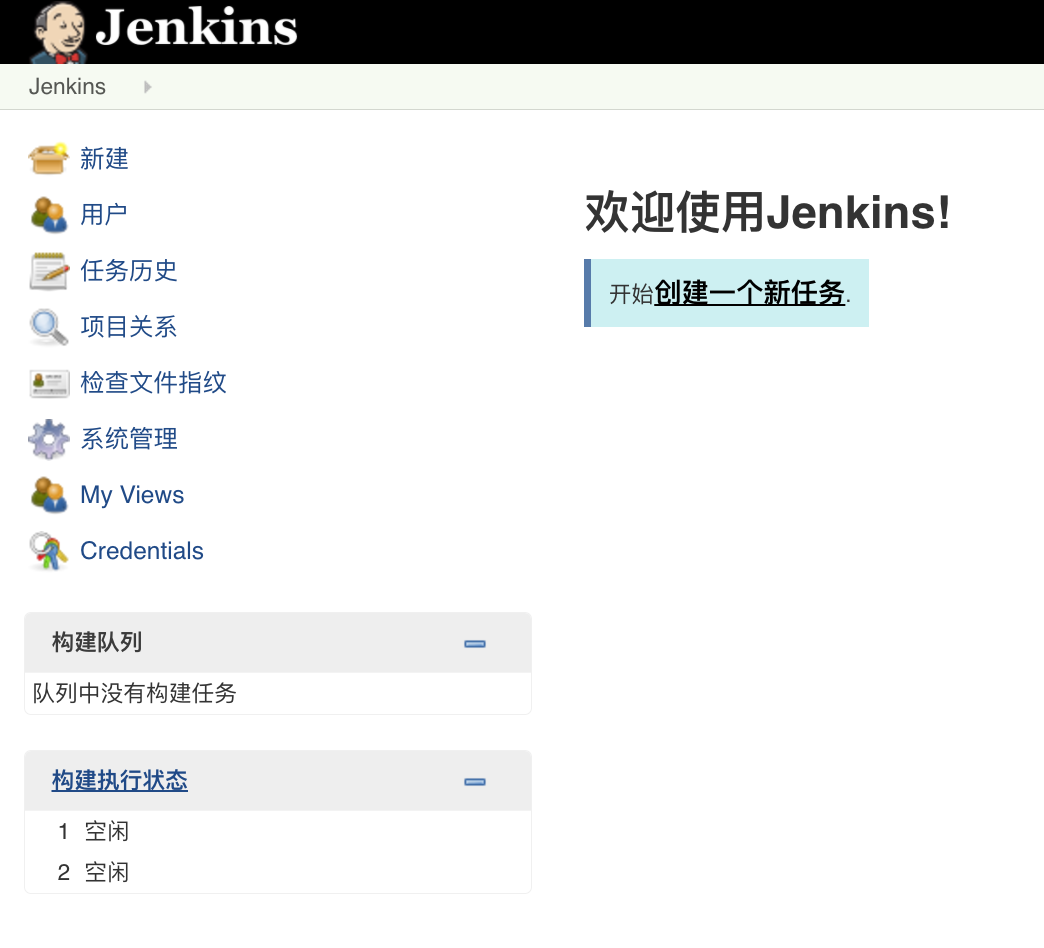
\includegraphics[width=5in]{chap02/jenkins3}
  \caption{Jenkins使用界面}
  \label{fig:jenkins3}
\end{figure}
% \begin{enumerate}
% \item 访问 http://mirrors.jenkins.io/war-stable/2.7.1/jenkins.war 下载2.7.1版本的jenkins安装包。
% \item 将jenkins.war 文件放到本地构建服务器(10.18.8.19)的Tomcat应用目录(/opt/tomcat/apache-tomcat-7.0.68/webapps)中。
% \item 配置并启动Tomcat即可完成安装,端口配置为8080,启动命令配置为:
% \begin{lstlisting}[language=bash,numbers=none]
% systemctl start/stop/status tomcat_jenkins.service
% \end{lstlisting}
% \item 访问jenkins地址(http://10.18.8.19:8080/jenkins/)初始化Jenkins:
% \begin{itemize}
% \item 完成认证,按照页面提示,将对应文件内容中的密码输入到文本框中,点击continue,如图\ref{fig:jenkins1}所示
% \begin{figure}[H] % use float package if you want it here
%   \centering
%   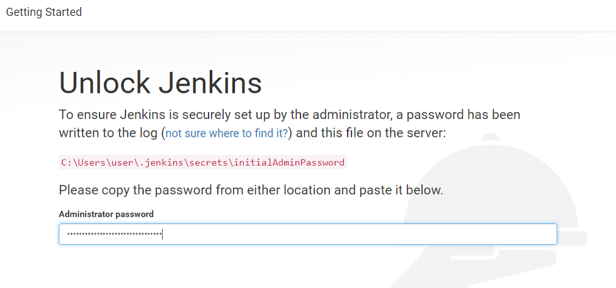
\includegraphics[width=5in]{chap02/jenkins1}
%   \caption{认证Jenkins界面}
%   \label{fig:jenkins1}
% \end{figure}
% \item 在插件选择处选择安装建议的插件
% \item 安装完成后在新的页面中配置用户名和密码完成安装,如图\ref{fig:jenkins2}
% \begin{figure}[H] % use float package if you want it here
%   \centering
%   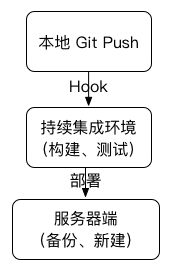
\includegraphics[width=5in]{chap02/jenkins2}
%   \caption{创建用户名和密码}
%   \label{fig:jenkins2}
% \end{figure}
% \item 进入图\ref{fig:jenkins3}页面表示安装成功
% \begin{figure}[H] % use float package if you want it here
%   \centering
%   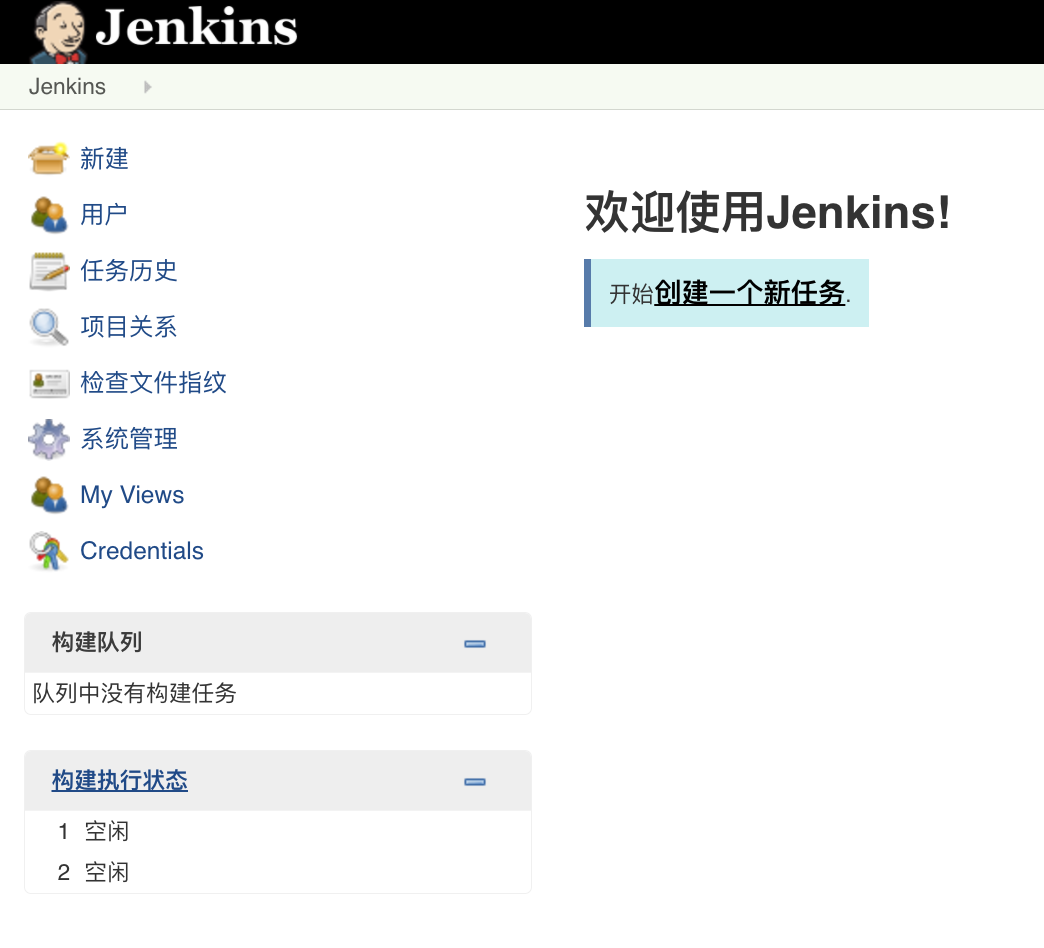
\includegraphics[width=5in]{chap02/jenkins3}
%   \caption{Jenkins使用界面}
%   \label{fig:jenkins3}
% \end{figure}
% \end{itemize}
% \end{enumerate}
\subsection{自动构建及检查方案设计}

由于小微平台通过Maven工具来解决代码使用过程中的函数依赖和本地项目构建\cite{董晓光2014使用},所以在进行自动构建的时候同样可以通过使用Maven Integration plugin插件实现项目的构建和代码检查,另外由于小微平台在开发过程中使用SVN来进行代码的版本控制,因此也需要在Jenkins中配置SVN插件来进行代码的同步和版本管理,除此之外,需要在安装Jenkins的服务器中提前安装好Maven软件。

小微项目在开发过程中是通过前后端分离进行的开发,因此在构建过程中需要新建前端项目和后端项目,考虑到前端项目的构建相对后端项目比较简单,本论文只介绍后端项目的创建和构建过程。
\begin{itemize}
  \item 新建Jenkins项目
  \begin{enumerate}
    \item 在Jenkins主页面新建项目后,首先填写项目名称(以ServerDeployforPROD1.2为例)
    \item 源码管理配置为SVN,具体如图\ref{fig:jenkins4}所示:
      \begin{figure}[H] % use float package if you want it here
        \centering
        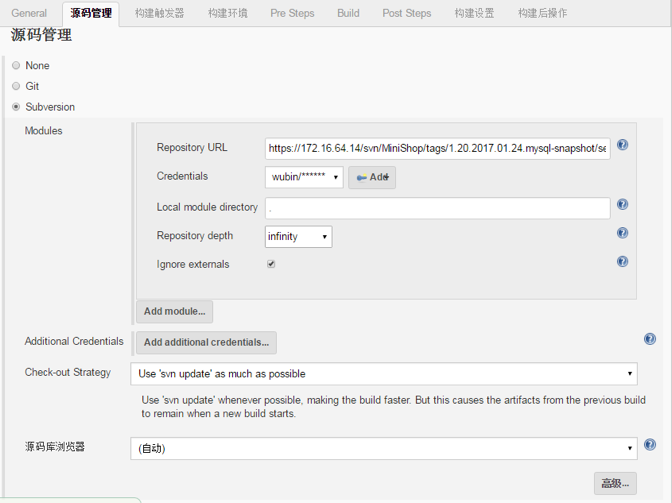
\includegraphics[width=6in]{chap02/jenkins4}
        \caption{Jenkins SVN配置}
        \label{fig:jenkins4}
      \end{figure}
      在对应的框中填写代码库的地址、通过Add按钮实现SVN的权限认证,其它选项选择默认即可。
    \item 在Pre Steps处增加shell命令为:
\begin{lstlisting}[language=bash,numbers=none]
rm -rf target/MiniShop
\end{lstlisting}
      确保每次构建时清除前一次构建信息。
    \item 在build标签页下配置构建时的操作,主要包括配置POM文件(pom.xml)的位置,pom.xml文件主要描述本Maven工程的整个生命周期所需要执行的功能和特性\cite{mileva2009mining},考虑到本项目的实际开发过程在这里选择项目pom2.xml
    \item 在Post Steps配置构建完成后的操作,首先需要在"Run only if build succeeds or is unstable"处打勾,保证在只有构建成功后才执行构建完成后的操作,其次需要配置构建完成对文件的操作:
\begin{lstlisting}[language=bash,numbers=none]
cp target/MiniShop.war /data/test/server/PROD/V1.2/MiniShop1.2_$(date +%Y%m%d)_$BUILD_NUMBER.war && chmod 777 /data/test/server/PROD/V1.2/MiniShop1.2_$(date +%Y%m%d)_$BUILD_NUMBER.war
\end{lstlisting}
      通过上述命令将每次构建完成后的文件进行备份保存和修改相应权限。
  \end{enumerate}
  所有项目信息配置完成后保存即可。
  \item 构建Jenkins项目

  进入项目主页,在页面左侧点击“立即构建”按钮即可进行构建,构建完成后将构建完成的war包上传到服务器即可,如果构建失败则表示在代码的书写过程中存在错误或者项目其他方面存在异常,需要在项目的构建信息页面中查看错误信息,并且根据错误信息来解决问题。
\end{itemize}

\subsection{自动部署方案设计}

Jenkins自动部署的方案是在每次构建完成后,让Jenkins可以自动的通过SSH协议访问远程服务器并将构建完成后的文件上传到服务器,并且执行服务器中的相应脚本来实现自动备份旧项目和部署新项目的目的。

\begin{enumerate}
  \item 在具体配置自动部署之前,需要先安装Publish Over SSH插件,通过这个插件,Jenkins可以实现通过SSH协议对远程服务器的访问。
  \item 在插件安装完成之后,需要配置插件来配置访问SSH的密钥和密码,在Jenkins“系统管理-系统设置”页面中会出现如图\ref{fig:jenkins5}配置:
    \begin{figure}[H] % use float package if you want it here
      \centering
      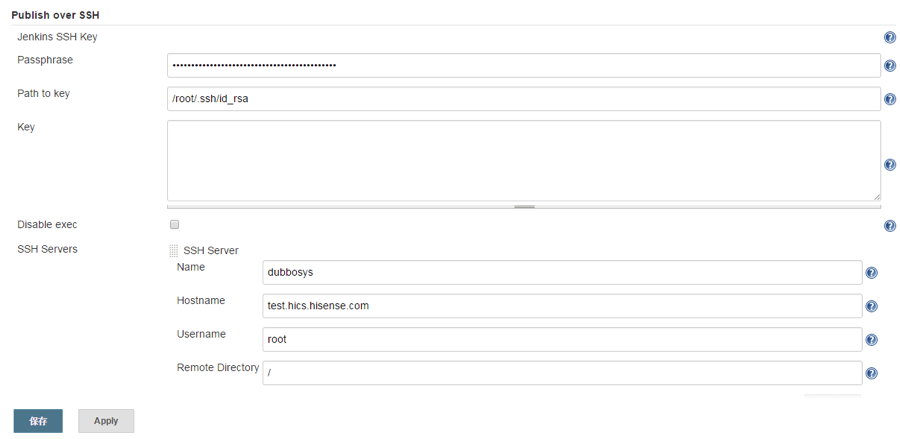
\includegraphics[width=6in]{chap02/jenkins5}
      \caption{Publish Over SSH插件配置}
      \label{fig:jenkins5}
    \end{figure}
  按照不同项目配置SSH Server信息和登录验证信息等。
  \item 插件配置完成后需要配置自动部署,插件安装完成后在“构建后操作”的选项中会出现“Send build artifacts over SSh”的选项,点击之后会出现配置:
    \begin{figure}[H] % use float package if you want it here
      \centering
      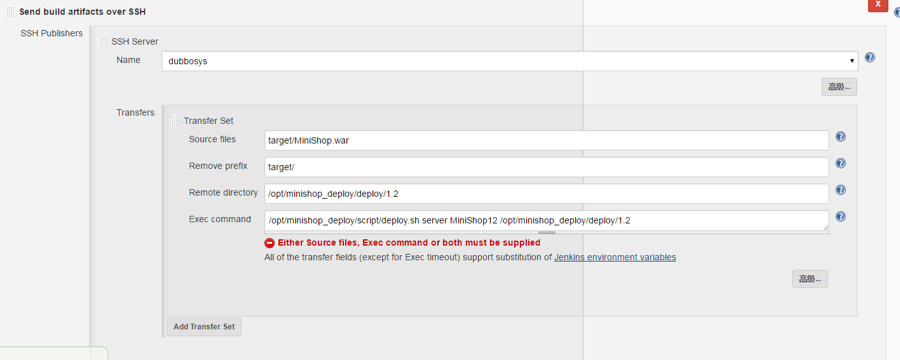
\includegraphics[width=7in]{chap02/jenkins6}
      \caption{Jenkins 自动部署配置}
      \label{fig:jenkins6}
    \end{figure}
  配置上传的文件名、上传后的路径、上传后需要执行的脚本和参数等,脚本可以参考附录\ref{cha:jenkinsdeploy}。
  \item 配置完成后再进行构建,Jenkins会自动的在构建后将构建生成的文件上传到服务器端指定路径,通过执行指定的脚本和参数将文件部署到Tomcat中,实现自动部署。
\end{enumerate}

\section{本章总结}

本章主要介绍了本人参与的小微项目的WEB平台所使用的开发框架、开发工具、开发过程以及系统上线的持续集成方案,通过持续集成方案增强了代码上线的稳定性,在本文后面的三章将会对本章开发的平台进行不同层级的优化,来实现本项目的安全性和高性能。